\label{exp:subqueries_joins}
\noindent
\begin{center}
    {\LARGE \textbf{DBMS LABORATORY PRACTICAL}}\\[0.25cm]
    \textbf{Practical No.:} 4 \hfill \textbf{Date:} 20/10/2026 \hfill \textbf{Page No.:} \thepage
\end{center}
\vspace{-0.2cm}
\hrule
\vspace{0.35cm}

\subsection*{Question / Problem Statement}
Design, implement, and execute nested subqueries and relational table joins on the \texttt{organisation} database using MySQL:
\begin{enumerate}[noitemsep,topsep=2pt]
    \item[(i)] Display employees earning more than the average salary.
    \item[(ii)] Display details of employees earning the minimum salary.
    \item[(iii)] Display all employees whose designation is identical to that of 'Arun'.
    \item[(iv)] Display employees who earn more than any employee in Department 1.
    \item[(v)] Display employee number, name, and department using \texttt{INNER JOIN}.
    \item[(vi)] Display employee details implementing a Left Outer Join (\texttt{LEFT OUTER JOIN}).
    \item[(vii)] Display employee details implementing a Right Outer Join (\texttt{RIGHT OUTER JOIN}).
\end{enumerate}

\vspace{0.25cm}
\subsection*{1. Single-Row Subqueries (Queries i, ii, iii)}

\subsubsection*{SQL Query}
\begin{lstlisting}[caption={Single-row subqueries using AVG, MIN, and attribute equality}]
USE organisation;

-- (i) Employees earning higher than the average salary
SELECT emp_no, emp_name, salary FROM employee
WHERE salary > (SELECT AVG(salary) FROM employee);

-- (ii) Details of employees earning the minimum salary
SELECT * FROM employee 
WHERE salary = (SELECT MIN(salary) FROM employee);

-- (iii) All employees sharing the same designation as 'Arun'
SELECT * FROM employee
WHERE designation = (
    SELECT designation FROM employee WHERE emp_name = 'Arun'
);
\end{lstlisting}

\newpage

\subsubsection*{Output Screenshot}
\begin{figure}[H]
    \centering
    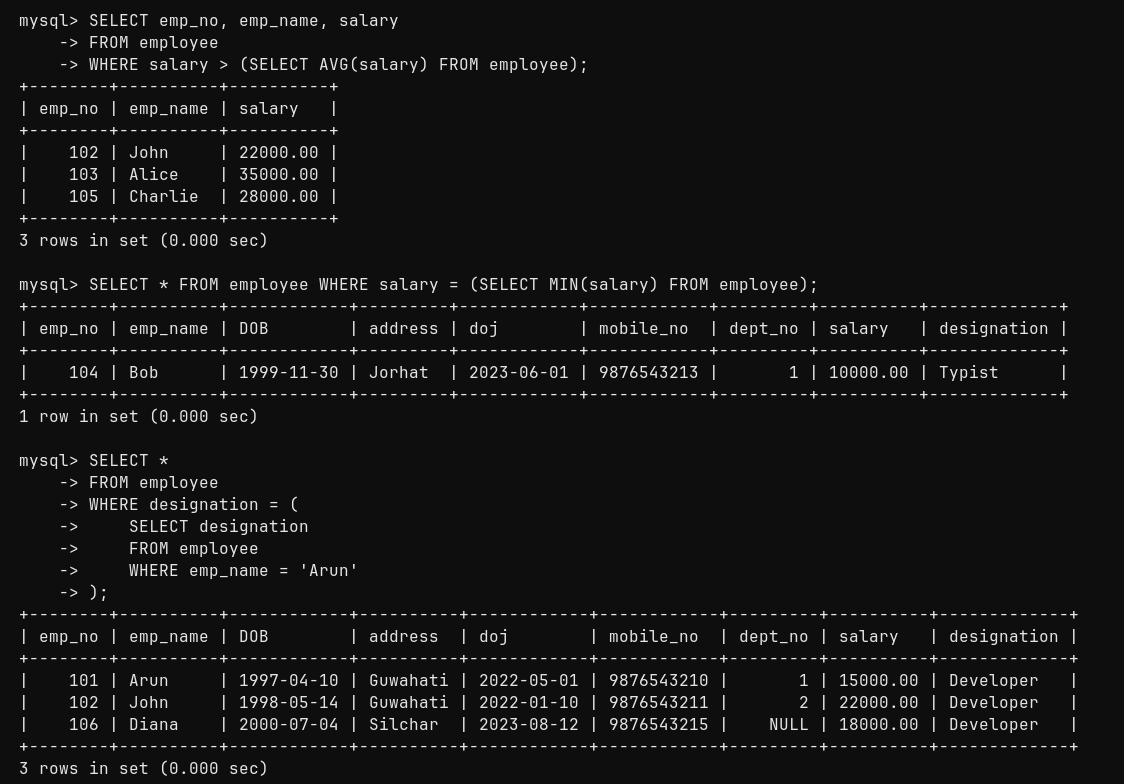
\includegraphics[width=0.92\linewidth,height=10.5cm,keepaspectratio]{Exp4-1.png}
    \caption{Single-row subqueries: employees above average salary, minimum salary, and matching designation.}
    \label{fig:exp4_subqueries_single}
\end{figure}

\newpage

\subsection*{2. Multi-Row Subquery \& Table Joins (Queries iv, v, vi, vii)}

\subsubsection*{SQL Query}
\begin{lstlisting}[caption={Multi-row subquery with ANY and table joins (INNER, LEFT, and RIGHT)}]
-- (iv) Employees earning more than any employee in Department 1
SELECT emp_no, emp_name FROM employee
WHERE salary > ANY (SELECT salary FROM employee WHERE dept_no = 1);
-- (v, vi) INNER JOIN and LEFT OUTER JOIN with department
SELECT e.emp_no, e.emp_name, d.dept_name
FROM employee e INNER JOIN department d ON e.dept_no = d.dept_no;
SELECT e.emp_no, e.emp_name, e.salary, d.dept_name
FROM employee e LEFT OUTER JOIN department d ON e.dept_no = d.dept_no;
-- (vii) RIGHT OUTER JOIN preserving unassigned departments
SELECT e.emp_no, e.emp_name, e.salary, d.dept_name
FROM employee e RIGHT OUTER JOIN department d ON e.dept_no = d.dept_no;
\end{lstlisting}

\subsubsection*{Output Screenshot}
\vspace{0.15cm}
\noindent\begin{minipage}[t]{0.48\textwidth}
    \centering
    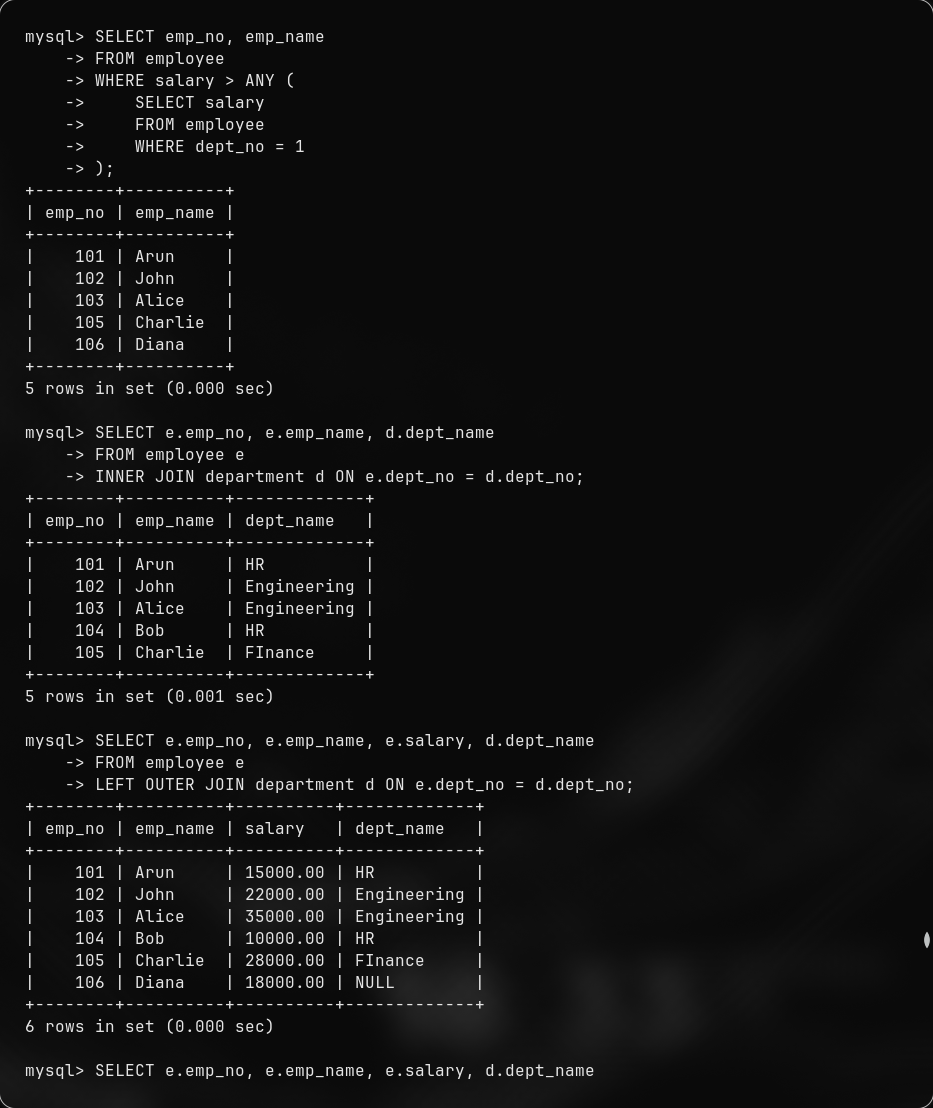
\includegraphics[width=\linewidth,height=7.2cm,keepaspectratio]{Exp4-2.png}
    \captionof{figure}{Queries iv, v, vi: \texttt{ANY}, Inner \& Left Join.}
    \label{fig:exp4_any_leftjoin}
\end{minipage}\hfill
\begin{minipage}[t]{0.48\textwidth}
    \centering
    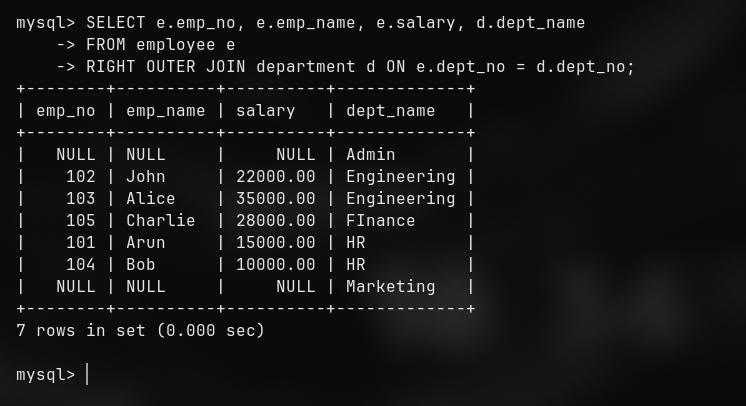
\includegraphics[width=\linewidth,height=4.2cm,keepaspectratio]{Exp4-3.png}
    \captionof{figure}{Query vii: Right Outer Join.}
    \label{fig:exp4_rightjoin}
\end{minipage}

\vspace{0.35cm}
\noindent\textbf{Result / Observation:}\quad The single-row subqueries, multi-row subqueries using \texttt{ANY}, and relational joins (\texttt{INNER JOIN}, \texttt{LEFT OUTER JOIN}, \texttt{RIGHT OUTER JOIN}) were executed successfully in MySQL.
